\documentclass{article}

\usepackage{graphicx}
\usepackage{hyperref}
\usepackage{tikz}
\usepackage{pgfplots}
\usepackage{multirow}
\usepackage{lipsum}
\usepackage{listings}
\usepackage{color}
\pgfplotsset{compat=1.16}
\pgfplotsset{width=10cm}


\author{Roșu Cristian-Mihai}
\title{HW2 Report}

\definecolor{dkgreen}{rgb}{0,0.6,0}
\definecolor{gray}{rgb}{0.5,0.5,0.5}
\definecolor{mauve}{rgb}{0.58,0,0.82}

\begin{document}

\lstset{frame=tb,
  language=C++,
  aboveskip=3mm,
  belowskip=3mm,
  showstringspaces=false,
  columns=flexible,
  basicstyle={\small\ttfamily},
  numbers=none,
  numberstyle=\tiny\color{gray},
  keywordstyle=\color{blue},
  commentstyle=\color{dkgreen},
  stringstyle=\color{mauve},
  breaklines=true,
  breakatwhitespace=true,
  tabsize=3
}

\maketitle

\begin{abstract}
Genetic algorithms have a lot of properties that make them a good choice when 
one needs to solve very complicated problems, however heuristics are 
powerful alternatives. One such problem is finding the global minima/maxima 
of multidimensional functions.

This work explores the efficiency of a genetic algorithm when dealing with
exactly this problem and comparing it to two of the most representative
heuristic search methods: Iterated Hillclimbing and Simulated Annealing.
\end{abstract}

\section{Introduction}
In computer science and operations research, a genetic algorithm (GA) is a 
metaheuristic inspired by the process of natural selection that belongs to 
the larger class of evolutionary algorithms (EA). Genetic algorithms are 
commonly used to generate high-quality solutions to optimization and search 
problems by relying on bio-inspired operators such as mutation, crossover and 
selection. \cite{ga}

This work aims to explore the capabilities of such a genetic algorithm to
generate solutions for the problem of searching for the global minimum of
a multidimensional function.

Here, \textit{Rastrigin}'s, \textit{Rosenbrock}'s, \textit{De Jong}'s and 
\textit{Michalewicz}'s functions are used as benchmarks to test a simple
genetic algorithm. Below are the functions \cite{functions}, in order:
$$ f(x) = A \cdot n + \sum_{i=1}^n \left[ x_i^2 - A \cdot cos(2 \pi x_i) \right], A = 10, x_i \in \left[ -5.12, 5.15 \right] $$
$$ f(x) = \sum_{i=1}^{n-1} \left[ 100({x_i}^2-x_{i+1})^2+(x_i-1)^2 \right], x_i \in \left[ -5, 10 \right]$$
$$ f(x) = \sum_{i=1}^n {x_i}^2, x_i \in \left[ -5.12, 5.12 \right] $$
$$ f(x) = - \sum_{i=1}^n \left[ \sin(x_i^2) \cdot \sin \left( \frac{i{x_i}^2}{\pi} \right)^{2m} \right], m = 10, x_i \in \left[ 0, \pi \right] $$
Being multidimensional, each of the functions will be tested on 5, 10 and 30 
dimensions, and for every test the \textsl{minimum}, \textsl{maximum} and 
\textsl{average} \textbf{values} found, as well as the \textsl{minimum}, 
\textsl{maximum} and \textsl{average} \textbf{time} it took to obtain those 
results will be recorded.

\subsection{Motivation} 
The purpose of this work is to explore the capabilities of a genetic algorithm.

In that sense, the problem of finding a function's global minimum has been 
chosen due to its ease of implementation and of understanding on a theoretical 
level. And as for the algorithms chosen, Iterated Hillclimbing and Simulated 
Annealing are the cornerstones of what genetics represents in computer 
science, on top of being equally easy to understand and implement. As such,
they are the perfect candidates to be compared to a genetic algorithm.

The benchmark functions have been chosen such that the experiment may include 
as much variety as possible, since the domain and global minimum of each of 
them are very distinct.

\section{Method}
In order to find the global minimum of a function, we use a simple genetic
algorithm and incorporate said function into the algorithm.

This is the general structure of a genetic algorithm:

\begin{lstlisting}
population <- vector(popSize, randomVector(d * L));
while (! STOP_CONDITION) {
    mutation(population);
    crossover(population);
    population <- selection(population, f());
}
\end{lstlisting}

By trying to imitate nature, a genetic algorithm considers the representation
of a population and emulates evolution across a certain number of generations
from which to extract solutions to the problem at hand.

In this case, the population is represented in a bitstring that is initially 
randomly generated called \texttt{population} whose size depends on the number of 
individuals in the population, or \textit{cromozomes}, and the length of their 
representation, a bitstring as well. The number of cromozomes used is 100.

After that, in order to manufacture the solution, the genetic operators are
applied to the population:

\begin{itemize}
\item \textbf{Mutation} - each bit in \texttt{population} has the low chance
of \textbf{0.01} of being inverted in order to increase diversity in the 
population and eliminate the posibility of stagnation.
\item \textbf{Crossover} - the operator with the biggest impact since it adds
new cromozomes in the population. Each cromozome is given a random chance, from
0 to 1. They are then sorted according to this chance and paired. The pairs
whose chances are lower than \textbf{0.3}, the chance for crossover, participate 
in crossover and create 2 new cromozomes by interchanging bits after a 
randomly chosen \textit{cutpoint}.
\item \textbf{Selection} - the operator that chooses the cromozomes that will
be part of the next generation. In order to determine that, a fitness is
calculated for each of the cromozomes. That fitness is where the optimization
function comes into play since the cromozome whose function evaluation is 
of lower value has a better fitness. That fitness is calculated with the
following formula:

\texttt{fitness($x_i$) <- 1.1 * max - f($x_i$), $\forall x_i$ cromozome}

where \texttt{max} is the maximum function value out of all the cromozomes in
the current generation and \texttt{f()} is the optimization function.

The process of choosing a candidate to go into the next generation is done
using the \textbf{Roulette Wheel} method coupled with \textbf{elitism}: the 
first \textbf{5} cromozomes with the best fitness are carried over and the 
rest are chosen randomly using a probabilty field that favours the cromozomes 
with high fitness.
\end{itemize}

These operations are performed on the population until a certain condition is
met. In this case, the stop condition is when the population reaches
its \textbf{250th generation}. The best cromozome out of all the generations
is the \textit{global minimum} found by the algorithm.

\section{Experiment}
The experiment consists in running the genetic algorithm through each of the 
benchmark functions on \textbf{5}, \textbf{10} and \textbf{30} dimensions, over \textbf{15 iterations}, in order 
to get a sample big enough to compare them by looking at the minimum, maximum 
and average \textit{values} produced, and the minimum, maximum and average \textit{times} it 
took to reach those values. In order to slightly speed up this process, the 
tests are run on two threads.

The performance of the genetic algorithm is then graphically compared to the
results of the previous experiment in HW1.

The code for this can be found on Github \cite{github}.
\section{Results}
Below are 4 tables corresponding to each of the 4 functions that hold the 
results to the experiment: Rastrigin, Rosenbrock, De Jong and Michalewicz, 
in that order.

\vspace{5mm}

\begin{figure}[!h]
  %\begin{table}[]
    \begin{tabular}{|l|l|l|l|l|}
        \hline
        \multicolumn{1}{|c|}{Method} & \multicolumn{1}{c|}{Dimension n} & \multicolumn{1}{c|}{5} & \multicolumn{1}{c|}{10} & \multicolumn{1}{c|}{30} \\ \hline
        \multirow{6}{*}{Genetic Algorithm} & Min & 0 & 4.5997 & 73.8115 \\ \cline{2-5} 
         & Max & 1.2481 & 11.4434 & 133.3624 \\ \cline{2-5} 
         & Average & 0.6240 & 6.3535 & 99.7060 \\ \cline{2-5} 
         & Min time & 212s & 413s & 1233s \\ \cline{2-5} 
         & Max time & 302s & 580s & 1769s \\ \cline{2-5} 
         & Average time & 288s & 560s & 1718s \\ \hline
    \end{tabular}
  %\end{table}
  \caption{Ratrigin's function results}
\end{figure}

\begin{figure}[!h]
  %\begin{table}[]
    \begin{tabular}{|l|l|l|l|l|}
        \hline
        \multicolumn{1}{|c|}{Method} & \multicolumn{1}{c|}{Dimension n} & \multicolumn{1}{c|}{5} & \multicolumn{1}{c|}{10} & \multicolumn{1}{c|}{30} \\ \hline
        \multirow{6}{*}{Genetic Algorithm} & Min & 0.0347 & 17.0955 & 4732.8138 \\ \cline{2-5} 
         & Max & 5.1822 & 193.9965 & 40878.7201 \\ \cline{2-5} 
         & Average & 2.0764 & 74.9848 & 14827.7693 \\ \cline{2-5} 
         & Min time & 200s & 431s & 1235s \\ \cline{2-5} 
         & Max time & 294s & 607s & 1819s \\ \cline{2-5} 
         & Average time & 283s & 584s & 1720s \\ \hline
    \end{tabular}
  %\end{table}
  \caption{Rosenbrock's function results}
\end{figure}

\begin{figure}[!h]
  %\begin{table}[]
    \begin{tabular}{|l|l|l|l|l|}
        \hline
        \multicolumn{1}{|c|}{Method} & \multicolumn{1}{c|}{Dimension n} & \multicolumn{1}{c|}{5} & \multicolumn{1}{c|}{10} & \multicolumn{1}{c|}{30} \\ \hline
        \multirow{6}{*}{Genetic Algorithm} & Min & 0 & 0.0028 & 3.0435 \\ \cline{2-5} 
         & Max & 0 & 0.0163 & 5.5702 \\ \cline{2-5} 
         & Average & 0 & 0.0087 & 4.1344 \\ \cline{2-5} 
         & Min time & 244s & 411s & 1285s \\ \cline{2-5} 
         & Max time & 335s & 599s & 3127s \\ \cline{2-5} 
         & Average time & 315s & 580s & 1898s \\ \hline
    \end{tabular}
  %\end{table}
  \caption{De Jong's function results}
\end{figure}

\begin{figure}[!h]
    %\begin{table}[]
        \begin{tabular}{|l|l|l|l|l|}
        \hline
        \multicolumn{1}{|c|}{Method} & \multicolumn{1}{c|}{Dimension n} & \multicolumn{1}{c|}{5} & \multicolumn{1}{c|}{10} & \multicolumn{1}{c|}{30} \\ \hline
        \multirow{6}{*}{Genetic Algorithm} & Min & -4.6879 & -9.4187 & -20.5711 \\ \cline{2-5} 
         & Max & 0 & 0 & 0 \\ \cline{2-5} 
         & Average & -4.5961 & -9.1553 & -19.4458 \\ \cline{2-5} 
         & Min time & 212s & 419s & 1213s \\ \cline{2-5} 
         & Max time & 291s & 575s & 1716s \\ \cline{2-5} 
         & Average time & 284s & 562s & 1637s \\ \hline
        \end{tabular}
    %\end{table}
  \caption{Michalewicz's function results}
\end{figure}

\newpage

And below are the graphs showing the difference in performance on 30 dimensions 
between the genetic algorithm and the heuristic search methods 
Iterated Hillclimbing and Simulated Annealing:

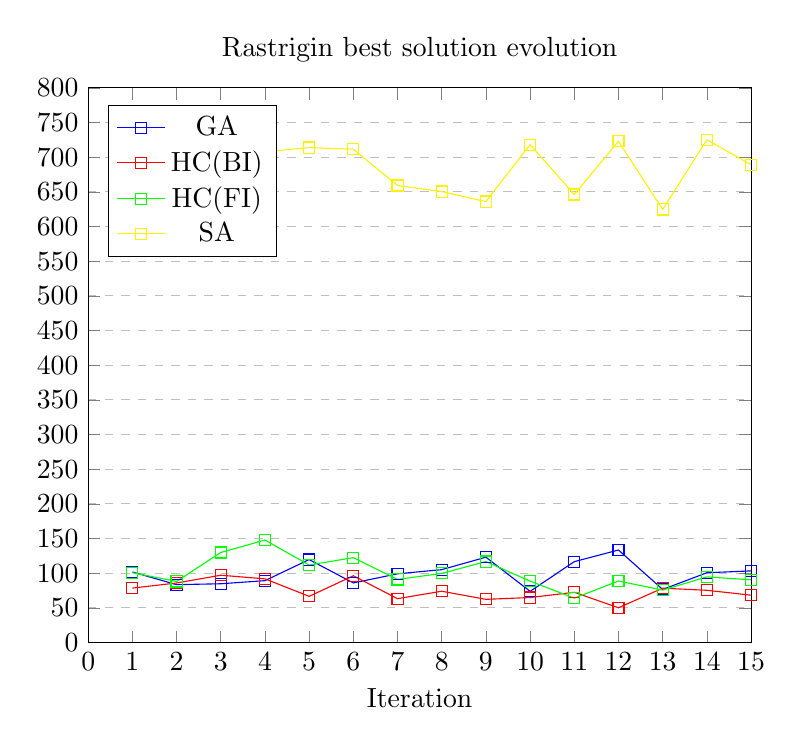
\begin{tikzpicture}
    \begin{axis}[
        title={Rastrigin best solution evolution},
        xlabel={Iteration},
        xmin=0, xmax=15,
        ymin=0, ymax=800,
        xtick={0,1,2,3,4,5,6,7,8,9,10,11,12,13,14,15},
        ytick={0,50,100,150,200,250,300,350,400,450,500,550,600,650,700,750,800},
        legend pos=north west,
        ymajorgrids=true,
        grid style=dashed,
    ]
     
    \addplot[
        color=blue,
        mark=square,
        ]
        coordinates {
        (1,101.6879)(2,83.3939)(3,84.6936)(4,89.1585)(5,119.5810)(6,85.8902)(7,99.0445)(8,105.0510)(9,122.9997)(10,73.8115)(11,116.5892)(12,133.3624)(13,76.5090)(14,100.5780)(15,103.2403)
        };
        \addlegendentry{GA}
     
    \addplot[
        color=red,
        mark=square,
    ]
    coordinates {
    (1,78.4602)(2,85.784)(3,97.0241)(4,91.7549)(5,66.5489)(6,96.1949)(7,63.1793)(8,73.9305)(9,62.2182)(10,64.8318)(11,72.3966)(12,50.0649)(13,78.3383)(14,75.2620)(15,68.2240)
    };
    \addlegendentry{HC(BI)}

    \addplot[
        color=green,
        mark=square,
    ]
    coordinates {
    (1,100.6540)(2,88.0193)(3,129.7700)(4,147.7450)(5,111.7750)(6,122.3430)(7,90.9444)(8,99.6295)(9,116.7460)(10,88.4789)(11,63.9453)(12,88.6400)(13,75.5550)(14,94.5970)(15,90.3883)
    };
    \addlegendentry{HC(FI)}

    \addplot[
        color=yellow,
        mark=square,
    ]
    coordinates {
    (1,631.7270)(2,760.1330)(3,579.8860)(4,707.6780)(5,713.9000)(6,711.5240)(7,659.1550)(8,650.4400)(9,635.9700)(10,718.188)(11,646.2010)(12,722.9340)(13,624.6470)(14,725.1080)(15,689.3350)
    };
    \addlegendentry{SA}

    \end{axis}
\end{tikzpicture}

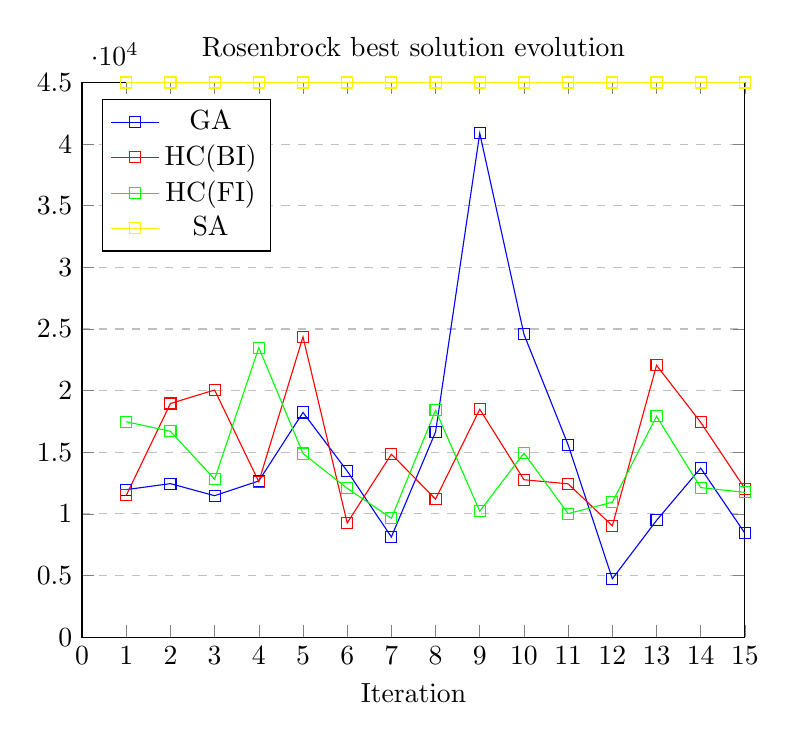
\begin{tikzpicture}
    \begin{axis}[
        title={Rosenbrock best solution evolution},
        xlabel={Iteration},
        xmin=0, xmax=15,
        ymin=0, ymax=45000,
        xtick={0,1,2,3,4,5,6,7,8,9,10,11,12,13,14,15},
        ytick={0,5000,10000,15000,20000,25000,30000,35000,40000,45000},
        legend pos=north west,
        ymajorgrids=true,
        grid style=dashed,
    ]
     
    \addplot[
        color=blue,
        mark=square,
        ]
        coordinates {
        (1,11965.1510)(2,12451.4769)(3,11471.8730)(4,12673.4937)(5,18226.5382)(6,13473.5753)(7,8124.0538)(8,16650.2084)(9,40878.7201)(10,24568.1128)(11,15595.4031)(12,4732.8138)(13,9467.7408)(14,13711.3611)(15,8426.0177)
        };
        \addlegendentry{GA}

    \addplot[
        color=red,
        mark=square,
        ]
        coordinates {
        (1,11496.5)(2,18953.6)(3,20051.3)(4,12606.0)(5,24360.5)(6,9260.82)(7,14841.1)(8,11197.1)(9,18484.6)(10,12767.9)(11,12436.2)(12,9032.11)(13,22052.0)(14,17424.9)(15,12037.8)
        };
        \addlegendentry{HC(BI)}
            
    \addplot[
        color=green,
        mark=square,
        ]
        coordinates {
        (1,17476.6)(2,16694.6)(3,12816.6)(4,23488.8)(5,14894.7)(6,12071.8)(7,9643.38)(8,18406.9)(9,10212.4)(10,14930.2)(11,10015.4)(12,10946.2)(13,17911.7)(14,12127.2)(15,11741.9)
        };
        \addlegendentry{HC(FI)}
            
    \addplot[
        color=yellow,
        mark=square,
        ]
        coordinates {
        (1,45000)(2,45000)(3,45000)(4,45000)(5,45000)(6,45000)(7,45000)(8,45000)(9,45000)(10,45000)(11,45000)(12,45000)(13,45000)(14,45000)(15,45000)
        };
        \addlegendentry{SA}
     
    \end{axis}
\end{tikzpicture}

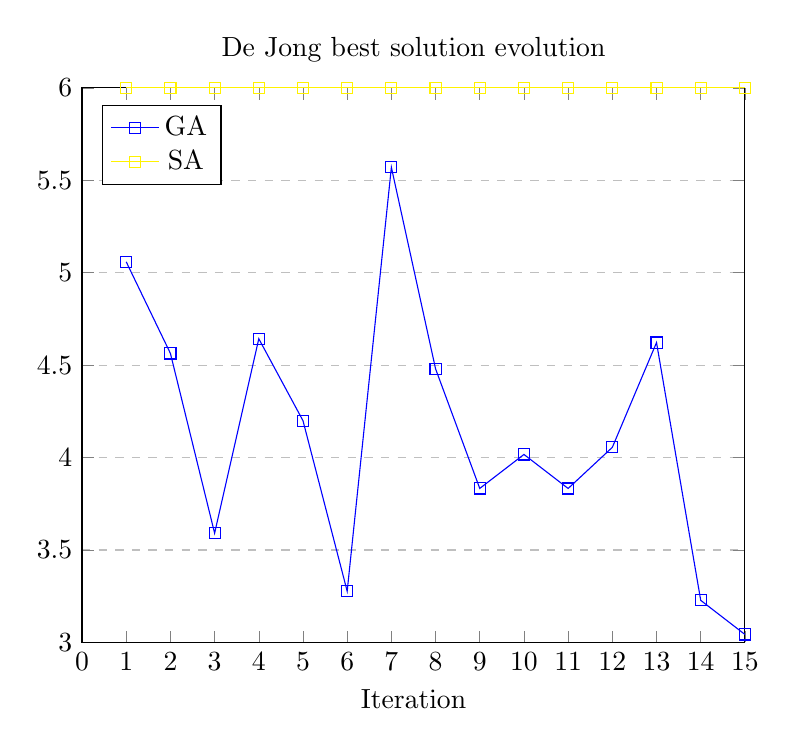
\begin{tikzpicture}
    \begin{axis}[
        title={De Jong best solution evolution},
        xlabel={Iteration},
        xmin=0, xmax=15,
        ymin=3, ymax=6,
        xtick={0,1,2,3,4,5,6,7,8,9,10,11,12,13,14,15},
        ytick={3,3.5,4,4.5,5,5.5,6},
        legend pos=north west,
        ymajorgrids=true,
        grid style=dashed,
    ]
     
    \addplot[
        color=blue,
        mark=square,
        ]
        coordinates {
        (1,5.0589)(2,4.5636)(3,3.5913)(4,4.6429)(5,4.1996)(6,3.2772)(7,5.5702)(8,4.4802)(9,3.8333)(10,4.0171)(11,3.8330)(12,4.0556)(13,4.6223)(14,3.2279)(15,3.0435)
        };
        \addlegendentry{GA}
        
    \addplot[
        color=yellow,
        mark=square,
        ]
        coordinates {
        (1,6)(2,6)(3,6)(4,6)(5,6)(6,6)(7,6)(8,6)(9,6)(10,6)(11,6)(12,6)(13,6)(14,6)(15,6)
        };
        \addlegendentry{SA}
     
    \end{axis}
\end{tikzpicture}

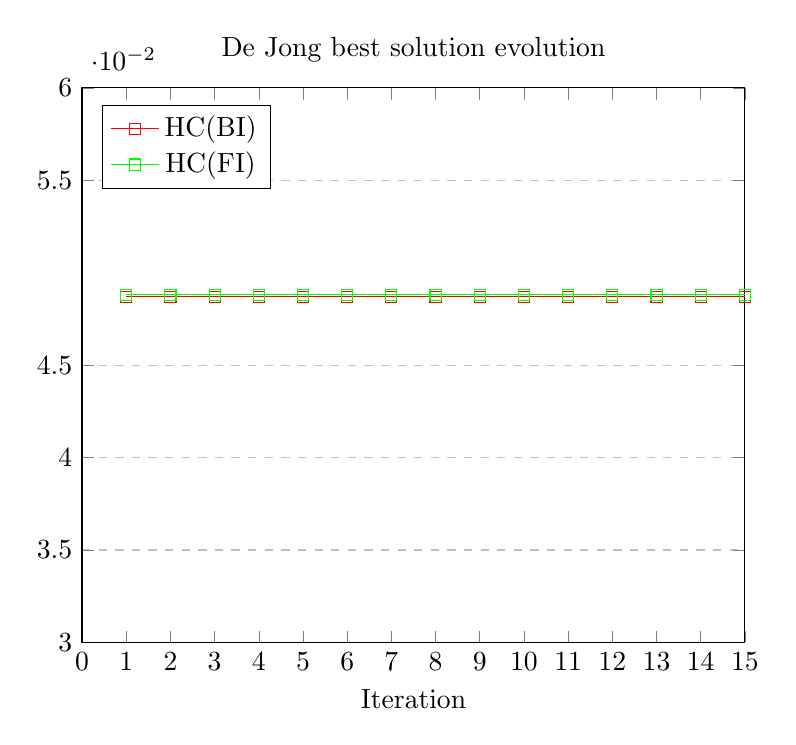
\begin{tikzpicture}
    \begin{axis}[
        title={De Jong best solution evolution},
        xlabel={Iteration},
        xmin=0, xmax=15,
        ymin=0.03, ymax=0.06,
        xtick={0,1,2,3,4,5,6,7,8,9,10,11,12,13,14,15},
        ytick={0.03,0.035,0.04,0.045,0.5,0.055,0.06},
        legend pos=north west,
        ymajorgrids=true,
        grid style=dashed,
    ]
  
    \addplot[
        color=red,
        mark=square,
        ]
        coordinates {
        (1,0.0487)(2,0.0487)(3,0.0487)(4,0.0487)(5,0.0487)(6,0.0487)(7,0.0487)(8,0.0487)(9,0.0487)(10,0.0487)(11,0.0487)(12,0.0487)(13,0.0487)(14,0.0487)(15,0.0487)
        };
        \addlegendentry{HC(BI)}
        
    \addplot[
        color=green,
        mark=square,
        ]
        coordinates {
        (1,0.0488)(2,0.0488)(3,0.0488)(4,0.0488)(5,0.0488)(6,0.0488)(7,0.0488)(8,0.0488)(9,0.0488)(10,0.0488)(11,0.0488)(12,0.0488)(13,0.0488)(14,0.0488)(15,0.0488)
        };
        \addlegendentry{HC(FI)}
     
    \end{axis}
\end{tikzpicture}

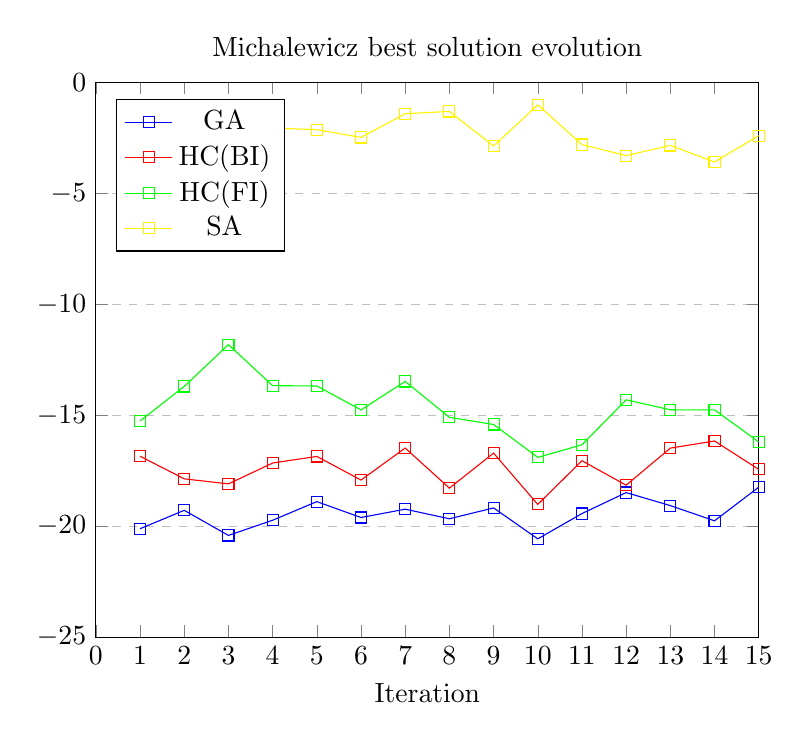
\begin{tikzpicture}
    \begin{axis}[
        title={Michalewicz best solution evolution},
        xlabel={Iteration},
        xmin=0, xmax=15,
        ymin=-25, ymax=0,
        xtick={0,1,2,3,4,5,6,7,8,9,10,11,12,13,14,15},
        ytick={-25,-20,-15,-10,-5,0},
        legend pos=north west,
        ymajorgrids=true,
        grid style=dashed,
    ]
     
    \addplot[
        color=blue,
        mark=square,
        ]
        coordinates {
        (1,-20.1140)(2,-19.2856)(3,-20.4169)(4,-19.7323)(5,-18.8934)(6,-19.6095)(7,-19.2341)(8,-19.6660)(9,-19.1770)(10,-20.5711)(11,-19.4303)(12,-18.4858)(13,-19.0734)(14,-19.7577)(15,-18.2410)
        };
        \addlegendentry{GA}

    \addplot[
        color=red,
        mark=square,
        ]
        coordinates {
        (1,-16.8453)(2,-17.8663)(3,-18.0931)(4,-17.1528)(5,-16.8552)(6,-17.9207)(7,-16.4774)(8,-18.2847)(9,-16.7066)(10,-19.0187)(11,-17.0489)(12,-18.1532)(13,-16.4801)(14,-16.1602)(15,-17.4395)
        };
        \addlegendentry{HC(BI)}
    
    \addplot[
        color=green,
        mark=square,
        ]
        coordinates {
        (1,-15.2565)(2,-13.7012)(3,-11.8155)(4,-13.6648)(5,-13.6810)(6,-14.7588)(7,-13.4747)(8,-15.0942)(9,-15.4147)(10,-16.8996)(11,-16.3322)(12,-14.3045)(13,-14.7536)(14,-14.7582)(15,-16.2026)
        };
        \addlegendentry{HC(FI)}
    
    \addplot[
        color=yellow,
        mark=square,
        ]
        coordinates {
        (1,-2.6807)(2,-1.9794)(3,-1.9135)(4,-2.0552)(5,-2.1267)(6,-2.4759)(7,-1.4072)(8,-1.3039)(9,-2.8624)(10,-1.0084)(11,-2.7991)(12,-3.2964)(13,-2.8364)(14,-3.5830)(15,-2.3956)
        };
        \addlegendentry{SA}
     
    \end{axis}
\end{tikzpicture}

\newpage

\section{Conclusions}
The genetic algorithm provides steadier and more consistent results, as oposed
to the two heuristic search algorithms. Across the 4 different function no
parameter changes have been made and still the solutions found and the time 
needed to reach them are fairly proportional. Additionaly, the genetic
algorithm has produced very good results on the lower dimensions.

On the other hand, it looses precision rather quickly as the dimension 
increases, and the times become a great deal longer, on top of already being
so compared to the alternatives.

\begin{thebibliography}{9}

\bibitem{ga}
    Wikipedia page for Genetic algorithm \\
    \url{https://en.wikipedia.org/wiki/Genetic_algorithm}

\bibitem{functions}
    Site with details of the functions used \\
    \url{http://www.geatbx.com/docu/fcnindex-01.html#P150_6749}

\bibitem{github}
    Github repository for the project \\
    \url{https://github.com/Nenma/ga-hw2}

\bibitem{pmihaela}
    Course site with the algorithms' details \\
    \url{https://profs.info.uaic.ro/~pmihaela/GA/laborator2.html}
  
\bibitem{tutorial}
    Simple Latex tutorial used \\
    \url{http://www.docs.is.ed.ac.uk/skills/documents/3722/3722-2014.pdf}

\bibitem{thesis}
    Thesis on GA Optimization used as reference \\
    \url{https://www.diva-portal.org/smash/get/diva2:832349/FULLTEXT01.pdf}

\end{thebibliography}
\end{document}
